\documentclass[11pt,a4paper]{article}

% ============================================================
% PAQUETS
% ============================================================
\usepackage[french]{babel}
\usepackage[utf8]{inputenc}
\usepackage[T1]{fontenc}
\usepackage[margin=2.5cm]{geometry}
\usepackage{graphicx}
\usepackage{booktabs}
\usepackage{array}
\usepackage{amsmath}
\usepackage{amssymb}
\usepackage{xcolor}
\usepackage{hyperref}
\usepackage{fancyhdr}
\usepackage{caption}
\usepackage{float}
\usepackage{enumitem}
\usepackage{listings}
\usepackage{tikz}
\usetikzlibrary{shapes,arrows.meta,positioning}

% ============================================================
% MISE EN PAGE
% ============================================================
\pagestyle{fancy}
\fancyhf{}
\fancyhead[L]{TP Traitement Numérique du Signal}
\fancyhead[R]{ENSET Douala -- Génie Informatique}
\fancyfoot[C]{\thepage}
\renewcommand{\headrulewidth}{0.4pt}

\hypersetup{
    colorlinks=true,
    linkcolor=blue!50!black,
    urlcolor=blue!50!black,
    citecolor=blue!50!black
}

\definecolor{codebg}{RGB}{245,245,245}
\lstset{
    backgroundcolor=\color{codebg},
    basicstyle=\ttfamily\small,
    breaklines=true,
    frame=single,
    numbers=left,
    numberstyle=\tiny,
    keywordstyle=\color{blue!70!black},
    commentstyle=\color{green!50!black},
}

\title{
    \vspace{-2cm}
    \begin{center}
        \textbf{UNIVERSITÉ DE DOUALA}\\
        \textbf{ENSET -- Département de Génie Informatique}\\
        \vspace{0.3cm}
        \rule{\linewidth}{0.5pt}
    \end{center}
    \vspace{0.5cm}
    \Large\textbf{Compte-rendu de Travaux Pratiques}\\
    \huge\textbf{Traitement Numérique du Signal}
}
\author{
    Rédigé par : Darix \\
    Niveau : 4 I.I / TIC \\
    Année académique : 2025--2026
}
\date{\today}

% ============================================================
% DOCUMENT
% ============================================================
\begin{document}

\maketitle
\thispagestyle{empty}

\begin{abstract}
\noindent
Ce document présente le compte-rendu complet du TP de Traitement Numérique du Signal (TNS). Il couvre l'analyse statistique d'un signal discret bruité, la conception et l'application de filtres numériques (FIR moyenne glissante, passe-haut, passe-bas), l'étude de sa transformée de Fourier discrète (TFD), ainsi que la conception d'une chaîne d'acquisition et de traitement embarquée sur ESP32 couplée à un dashboard web de supervision temps réel.
\end{abstract}

\vspace{0.5cm}
\noindent\textbf{Contexte :} Un système embarqué acquiert un signal analogique bruité provenant d'un capteur biomédical ou industriel. Le signal discret étudié est :
\[
x[n] = \{12, 15, 18, 22, 30, 28, 35, 40, 38, 45, 50, 48, 55, 60\}, \quad n = 0, \dots, 13
\]
Ce signal contient du bruit haute fréquence, des variations lentes et des perturbations impulsionnelles.

\newpage
\tableofcontents
\newpage

% ============================================================
% PARTIE A
% ============================================================
\section{Analyse du signal}

\subsection{Représentation du signal \texorpdfstring{$x[n]$}{x[n]}}

Le signal discret $x[n]$ est représenté ci-dessous.

\begin{figure}[H]
    \centering
    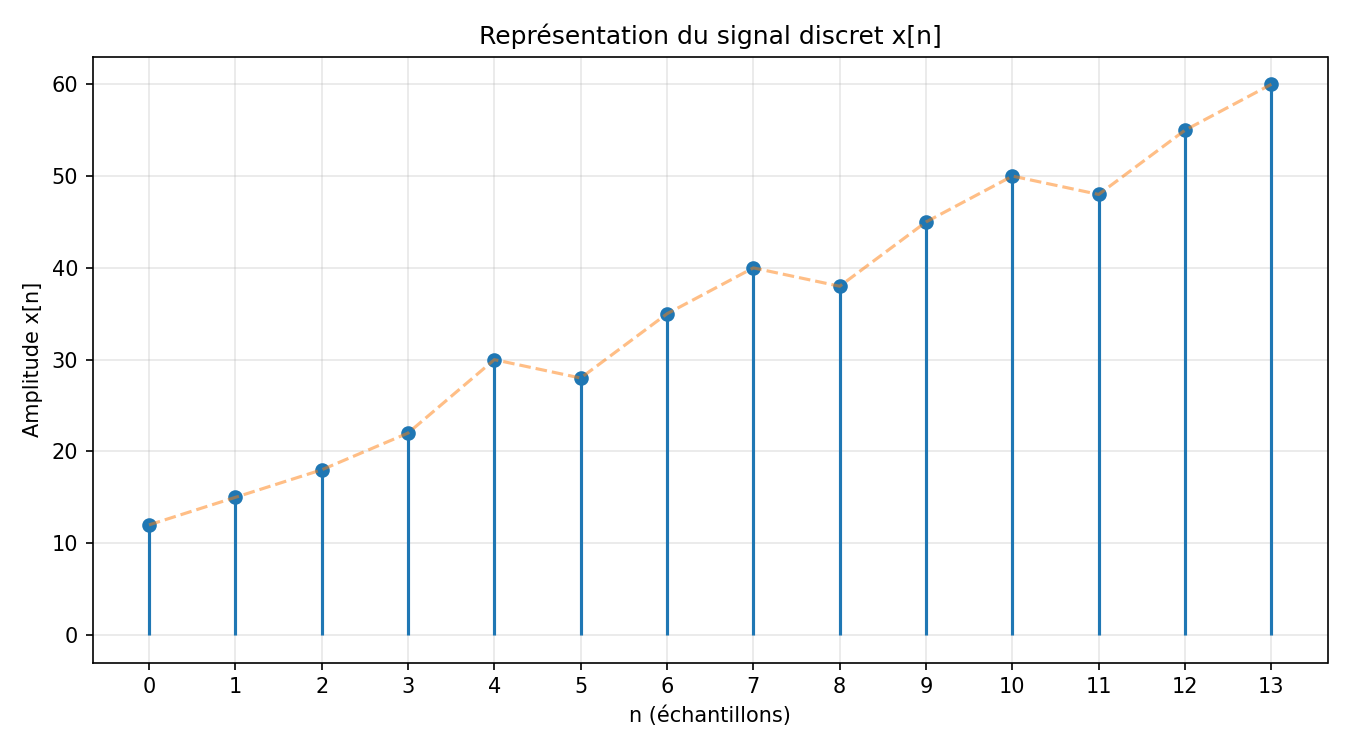
\includegraphics[width=0.75\textwidth]{signal_xn.png}
    \caption{Représentation temporelle du signal discret $x[n]$}
    \label{fig:signal_xn}
\end{figure}

\subsection{Grandeurs statistiques}

Les grandeurs statistiques du signal sont calculées à partir des $N = 14$ échantillons :

\[
\bar{x} = \frac{1}{N}\sum_{n=0}^{N-1} x[n], \qquad
\sigma^2 = \frac{1}{N}\sum_{n=0}^{N-1} (x[n] - \bar{x})^2
\]

\begin{table}[H]
    \centering
    \caption{Grandeurs statistiques du signal $x[n]$}
    \label{tab:stats_A}
    \begin{tabular}{@{}lc@{}}
        \toprule
        \textbf{Grandeur} & \textbf{Valeur} \\
        \midrule
        Nombre d'échantillons $N$          & 14 \\
        Moyenne $\bar{x}$                   & 35.429 \\
        Variance (biaisée, $/N$)            & 215.102 \\
        Variance (échantillon, $/(N-1)$)    & 231.648 \\
        Écart-type $\sigma$                 & 14.666 \\
        Amplitude maximale                  & 60 \\
        Amplitude minimale                  & 12 \\
        Étendue (max $-$ min)                & 48 \\
        \bottomrule
    \end{tabular}
\end{table}

\subsection{Commentaire sur la nature du signal}

Le signal est globalement croissant, révélant une \textbf{tendance de fond} (variation lente, de 12 à 60 sur la durée d'observation), mais présente des irrégularités locales -- par exemple la chute $22 \rightarrow 30 \rightarrow 28$ ou $45 \rightarrow 50 \rightarrow 48 \rightarrow 55$ -- qui traduisent la superposition d'un bruit haute fréquence et de perturbations impulsionnelles sur la tendance de base. L'écart-type élevé ($\sigma \approx 14.7$) par rapport à l'amplitude confirme une variabilité non négligeable, cohérente avec un capteur biomédical ou industriel bruité.

% ============================================================
% PARTIE B
% ============================================================
\newpage
\section{Filtrage numérique}

\subsection{Filtre FIR -- Moyenne glissante}

Le filtre FIR moyenne glissante d'ordre 4 est défini par :

\[
y[n] = \frac{1}{4}\sum_{k=0}^{3} x[n-k]
\]

avec la convention causale $x[n] = 0$ pour $n < 0$.

\subsubsection{5 premières valeurs filtrées}

\begin{table}[H]
    \centering
    \caption{5 premières valeurs du signal filtré par le FIR moyenne glissante}
    \label{tab:fir_5premieres}
    \begin{tabular}{@{}cc@{}}
        \toprule
        $n$ & $y[n]$ \\
        \midrule
        0 & 3.000 \\
        1 & 6.750 \\
        2 & 11.250 \\
        3 & 16.750 \\
        4 & 21.250 \\
        \bottomrule
    \end{tabular}
\end{table}

\subsubsection{Interprétation de l'effet sur le bruit}

Le filtre FIR moyenne glissante \textbf{lisse} le signal : la somme des variations absolues passe de 60 (signal brut) à environ 50.25 (signal filtré), soit une réduction de variabilité de \textbf{16.2\,\%}. Il atténue efficacement le bruit haute fréquence et les petites oscillations, au prix d'un léger retard de groupe et d'un lissage des transitions rapides.

\begin{figure}[H]
    \centering
    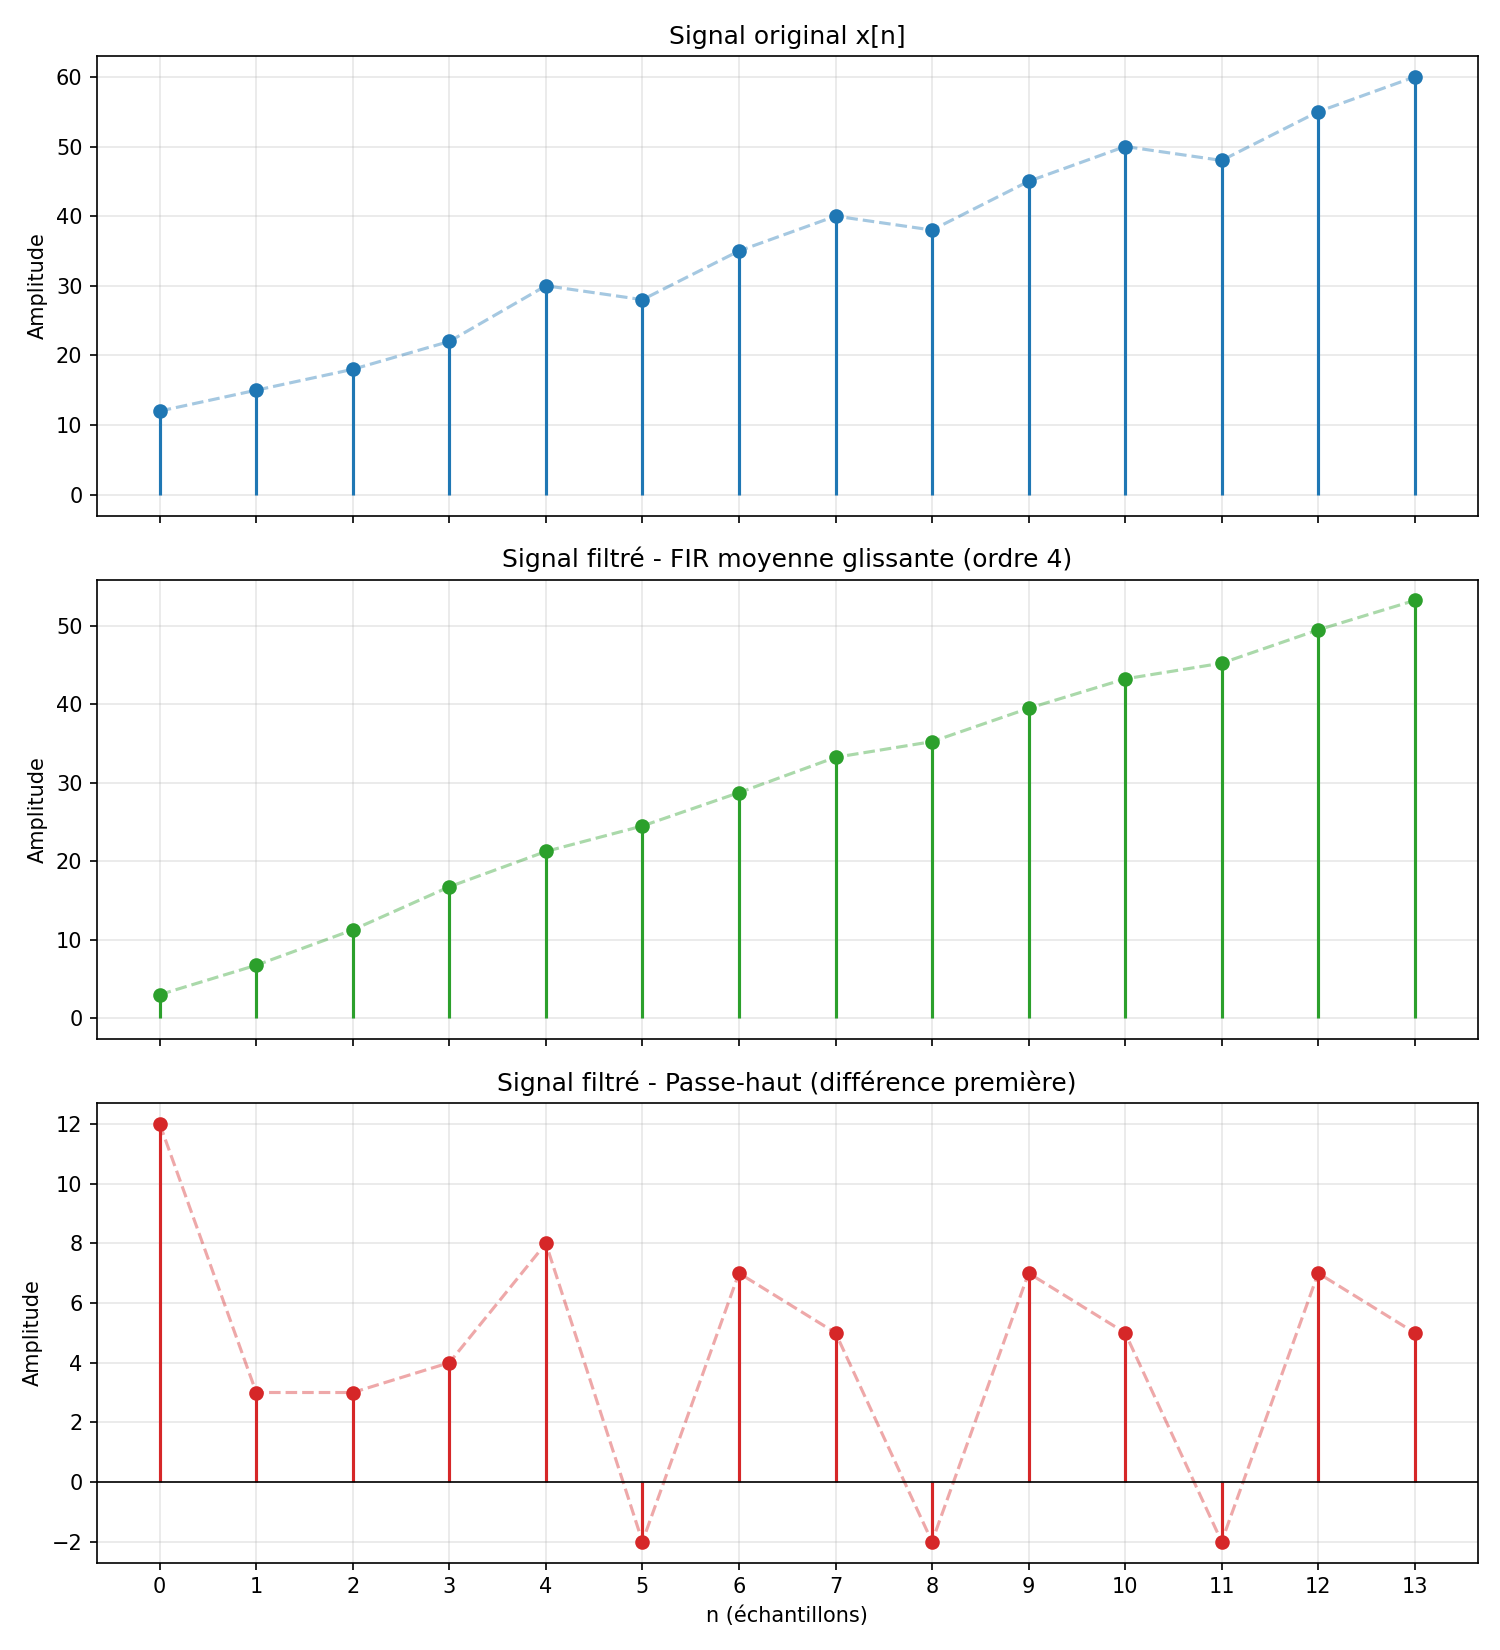
\includegraphics[width=0.85\textwidth]{partie_B_filtrage.png}
    \caption{Signal original, signal filtré FIR et signal filtré passe-haut}
    \label{fig:partie_B_filtrage}
\end{figure}

\begin{figure}[H]
    \centering
    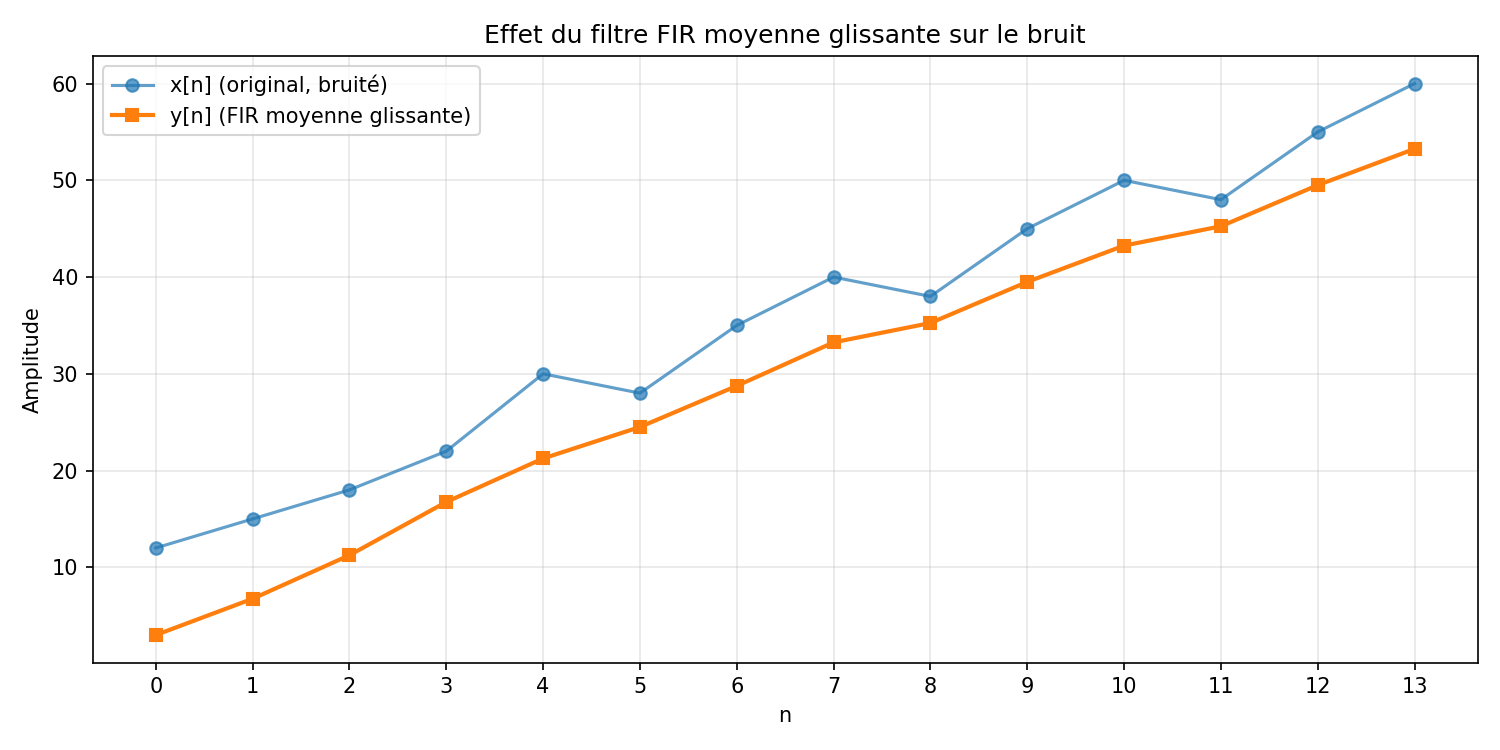
\includegraphics[width=0.8\textwidth]{partie_B_comparaison_fir.png}
    \caption{Comparaison superposée : effet du filtre FIR sur le bruit}
    \label{fig:partie_B_comparaison}
\end{figure}

\subsection{Filtre passe-haut}

Le filtre passe-haut (différence première) est défini par :

\[
y[n] = x[n] - x[n-1]
\]

\begin{table}[H]
    \centering
    \caption{Réponse du filtre passe-haut sur l'ensemble du signal}
    \label{tab:passe_haut}
    \begin{tabular}{@{}cccccccc@{}}
        \toprule
        $n$ & 0 & 1 & 2 & 3 & 4 & 5 & 6 \\
        $y_{HP}[n]$ & 12 & 3 & 3 & 4 & 8 & $-2$ & 7 \\
        \midrule
        $n$ & 7 & 8 & 9 & 10 & 11 & 12 & 13 \\
        $y_{HP}[n]$ & 5 & $-2$ & 7 & 5 & $-2$ & 7 & 5 \\
        \bottomrule
    \end{tabular}
\end{table}

\subsubsection{Mise en évidence des variations rapides}

Les plus fortes variations ($n=0$, $n=4$, $n=12$) correspondent aux discontinuités les plus marquées de $x[n]$. Le filtre passe-haut rejette la composante continue/lente et fait ressortir le bruit et les transitions brusques, à l'inverse du filtre FIR qui les atténue.

% ============================================================
% PARTIE C
% ============================================================
\newpage
\section{Transformation fréquentielle}

\subsection{La Transformée de Fourier Discrète (TFD)}

La TFD permet de passer de la représentation \textbf{temporelle} d'un signal discret $x[n]$ à sa représentation \textbf{fréquentielle} $X[k]$. Elle décompose le signal en une somme de sinusoïdes complexes de fréquences différentes, révélant quelles fréquences composent le signal et avec quelle amplitude/phase.

\[
X[k] = \sum_{n=0}^{N-1} x[n] \, e^{-j\frac{2\pi}{N}kn}, \qquad k = 0, 1, \dots, N-1
\]

\begin{itemize}[label=--]
    \item $X[k]$ : valeur complexe représentant l'amplitude et la phase de la composante fréquentielle $k$ ;
    \item $k=0$ : composante continue (moyenne du signal) ;
    \item $k$ petit : basses fréquences (tendances lentes) ;
    \item $k$ proche de $N/2$ : hautes fréquences (variations rapides, bruit).
\end{itemize}

En pratique, on l'implémente efficacement via la \textbf{FFT} (\emph{Fast Fourier Transform}, \texttt{numpy.fft.fft}).

\subsection{Identification des composantes basse et haute fréquence}

\begin{table}[H]
    \centering
    \caption{Spectre d'amplitude $|X[k]|$ du signal $x[n]$}
    \label{tab:spectre}
    \begin{tabular}{@{}cccl@{}}
        \toprule
        $k$ & Fréquence normalisée & $|X[k]|$ & Interprétation \\
        \midrule
        0 & 0.000 & 496.0 & Composante continue \\
        1 & 0.071 & 111.6 & Basse fréquence dominante \\
        2 & 0.143 & 59.7  & Basse fréquence secondaire \\
        3 & 0.214 & 40.4  & Fréquence intermédiaire \\
        4 & 0.286 & 33.5  & Fréquence intermédiaire \\
        5 & 0.357 & 38.6  & Fréquence intermédiaire/haute \\
        6 & 0.429 & 25.2  & Haute fréquence \\
        7 & 0.500 & 20.0  & Fréquence de Nyquist \\
        \bottomrule
    \end{tabular}
\end{table}

\begin{figure}[H]
    \centering
    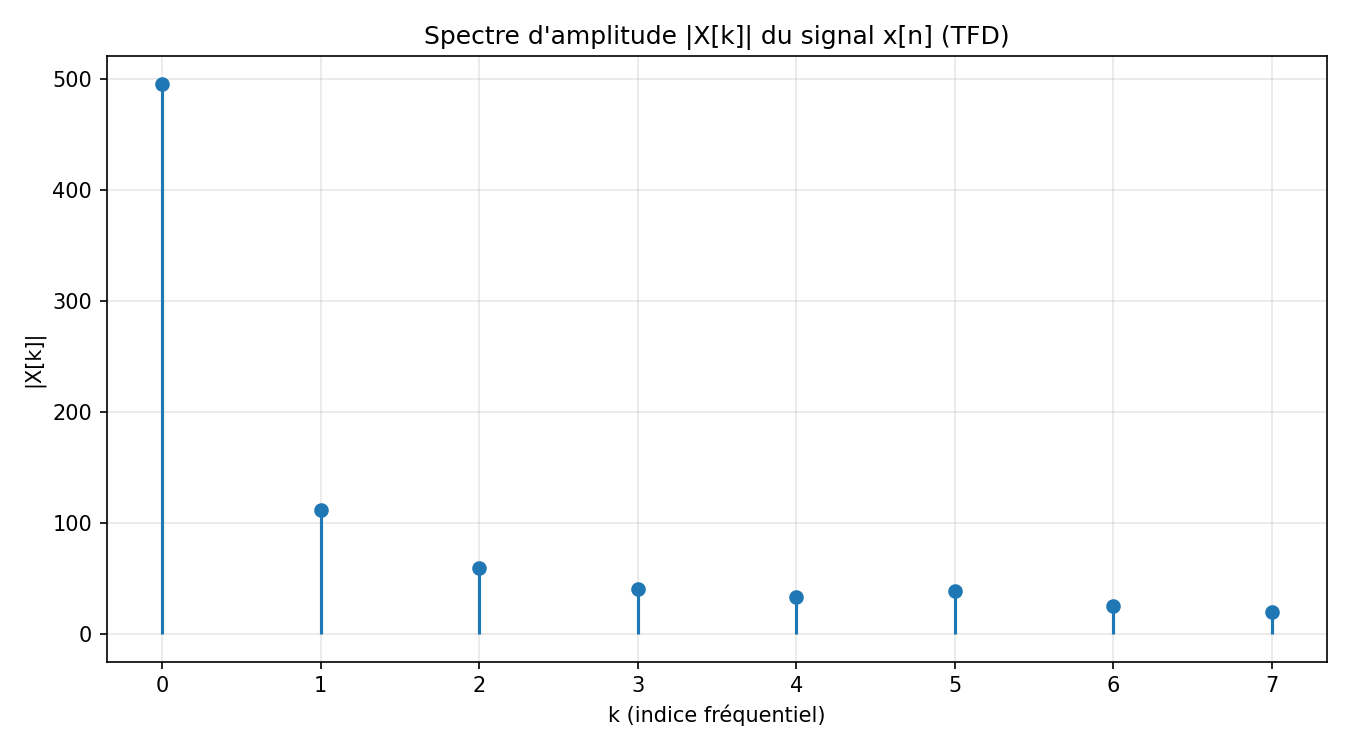
\includegraphics[width=0.8\textwidth]{partie_C_spectre.png}
    \caption{Spectre d'amplitude $|X[k]|$ obtenu par TFD}
    \label{fig:spectre}
\end{figure}

\textbf{Constat :} l'énergie est concentrée sur les premières raies ($k=0$ et $k=1$), confirmant que le signal est dominé par une tendance lente et croissante. Les composantes à $k \geq 5$, d'amplitude plus faible mais non négligeable, traduisent le bruit haute fréquence et les perturbations impulsionnelles superposés à la tendance de fond.

\subsection{Interprétation physique du spectre}

\begin{itemize}[label=--]
    \item Le \textbf{pic en $k=0$} représente le niveau moyen du signal (offset), lié à la ligne de base du capteur.
    \item Le \textbf{pic dominant en $k=1$} correspond à la variation physiologique/physique lente du phénomène mesuré.
    \item Les \textbf{composantes hautes fréquences} ($k=5$ à $7$) correspondent au bruit électronique de la chaîne d'acquisition et aux perturbations impulsionnelles ponctuelles.
    \item \textbf{Conclusion :} le signal utile se situe dans les basses fréquences, tandis que le bruit à filtrer se situe dans les hautes fréquences -- ce qui justifie l'usage d'un filtre passe-bas (Partie D).
\end{itemize}

% ============================================================
% PARTIE D
% ============================================================
\newpage
\section{Conception d'un filtre numérique}

\subsection{Équation temporelle}

Le filtre est donné par sa fonction de transfert en $z$ :

\[
H(z) = 0.5 + 0.5\,z^{-1}
\]

Sachant que $Y(z) = H(z)\cdot X(z)$ et que $z^{-1}$ correspond à un retard d'un échantillon, l'équation aux différences (équation temporelle) est :

\[
\boxed{y[n] = 0.5\,x[n] + 0.5\,x[n-1]}
\]

C'est un filtre RIF (FIR) d'ordre 1, à coefficients $h[0]=0.5$, $h[1]=0.5$ -- c'est-à-dire une moyenne glissante à 2 points.

\subsection{Réponse du filtre pour le signal donné}

\begin{table}[H]
    \centering
    \caption{Réponse du filtre $H(z) = 0.5 + 0.5z^{-1}$ pour le signal $x[n]$}
    \label{tab:reponse_D}
    \begin{tabular}{@{}ccc|ccc@{}}
        \toprule
        $n$ & $x[n]$ & $y[n]$ & $n$ & $x[n]$ & $y[n]$ \\
        \midrule
        0 & 12 & 6.0  & 7  & 40 & 37.5 \\
        1 & 15 & 13.5 & 8  & 38 & 39.0 \\
        2 & 18 & 16.5 & 9  & 45 & 41.5 \\
        3 & 22 & 20.0 & 10 & 50 & 47.5 \\
        4 & 30 & 26.0 & 11 & 48 & 49.0 \\
        5 & 28 & 29.0 & 12 & 55 & 51.5 \\
        6 & 35 & 31.5 & 13 & 60 & 57.5 \\
        \bottomrule
    \end{tabular}
\end{table}

\begin{figure}[H]
    \centering
    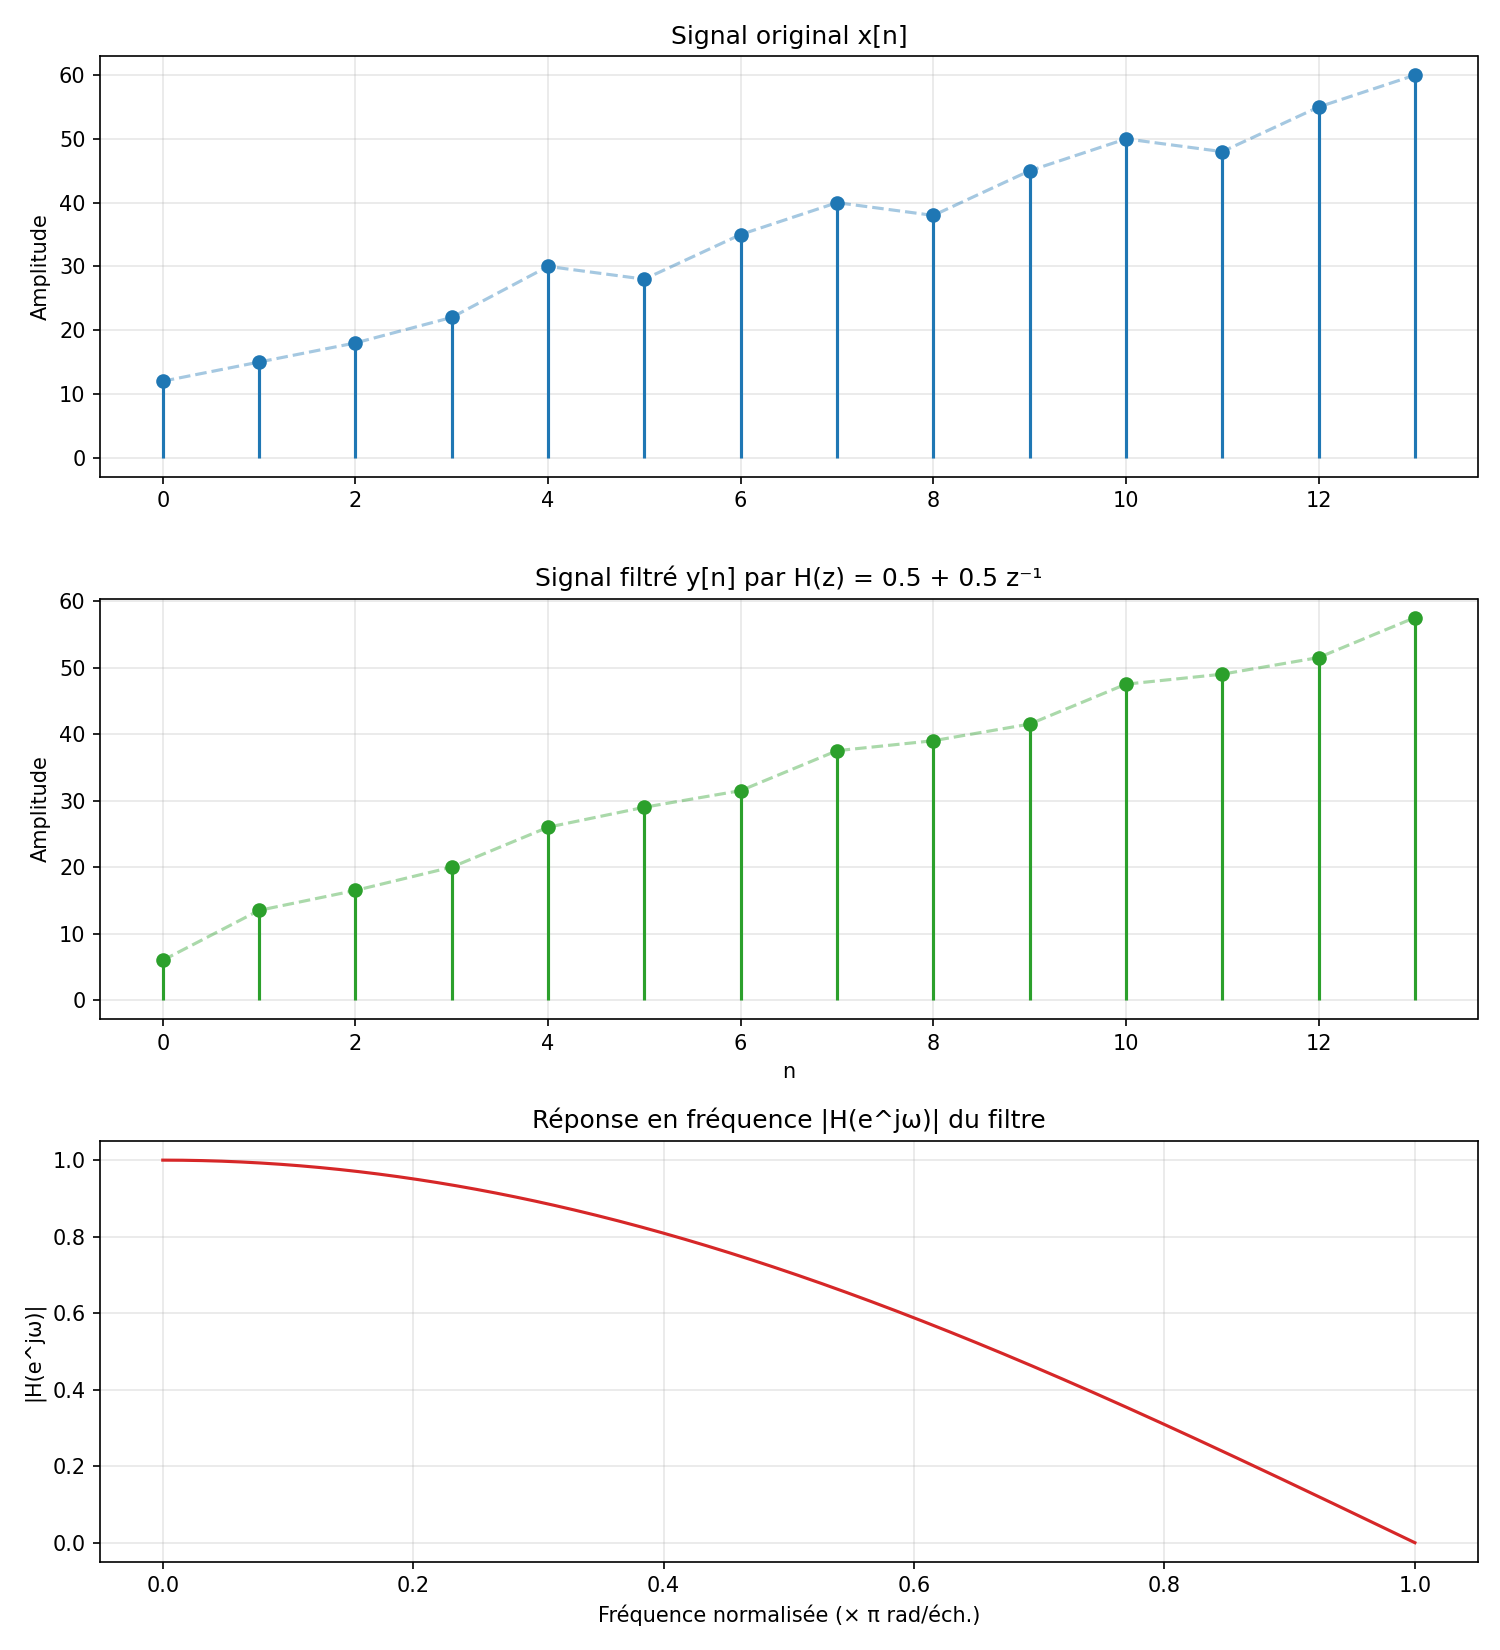
\includegraphics[width=0.85\textwidth]{partie_D_filtre.png}
    \caption{Signal original, signal filtré par $H(z)$ et réponse en fréquence $|H(e^{j\omega})|$}
    \label{fig:partie_D}
\end{figure}

\textbf{Vérification par la réponse en fréquence} $H(e^{j\omega}) = 0.5 + 0.5e^{-j\omega}$ :
\begin{itemize}[label=--]
    \item Gain en $\omega = 0$ (continu) : $|H(0)| = 1.0$ $\rightarrow$ aucune atténuation des basses fréquences ;
    \item Gain en $\omega = \pi$ (Nyquist) : $|H(\pi)| = 0.0$ $\rightarrow$ atténuation totale des hautes fréquences.
\end{itemize}
Ceci confirme le comportement \textbf{passe-bas} du filtre.

\subsection{Justification de son utilité}

\begin{itemize}[label=--]
    \item \textbf{Réduction de la variabilité} : la somme des variations absolues passe de 60 à 51.5, soit une réduction de \textbf{14.2\,\%}.
    \item \textbf{Comportement fréquentiel adapté} : d'après le spectre étudié en Partie C, l'information utile est concentrée en basse fréquence tandis que le bruit occupe les hautes fréquences. $H(z)$ élimine donc sélectivement le bruit tout en préservant la dynamique lente du signal.
    \item \textbf{Simplicité d'implémentation embarquée} : filtre FIR d'ordre 1, 2 coefficients égaux à $0.5$ -- une addition et un décalage binaire suffisent, ce qui le rend très adapté à un système embarqué temps réel (ESP32/Arduino).
    \item \textbf{Stabilité garantie} : étant un filtre FIR (pas de pôle, uniquement un zéro en $z=-1$), il est inconditionnellement stable, contrairement à un filtre récursif (IIR).
\end{itemize}

% ============================================================
% PARTIE E
% ============================================================
\newpage
\section{Implémentation embarquée}

\subsection{Architecture du système complet}

Le système complet proposé répond aux exigences d'acquisition temps réel, de filtrage adaptatif, de détection d'événements, de transmission vers Flask et d'affichage web.

\begin{figure}[H]
    \centering
    \begin{tikzpicture}[
        node distance=1.4cm and 2.2cm,
        block/.style={rectangle, draw, rounded corners, minimum width=3.2cm, minimum height=1cm, align=center, font=\small},
        arrowstyle/.style={-{Latex[length=2.5mm]}, thick}
    ]
        \node[block] (capteur) {Capteur\\analogique};
        \node[block, right=of capteur] (esp32) {ESP32\\Acquisition + Filtrage\\+ Détection};
        \node[block, right=of esp32] (flask) {Serveur Flask\\(API + SocketIO)};
        \node[block, right=of flask] (web) {Dashboard Web\\(Chart.js, temps réel)};
        \node[block, below=of esp32] (uart) {Moniteur série\\(UART, debug)};

        \draw[arrowstyle] (capteur) -- (esp32);
        \draw[arrowstyle] (esp32) -- node[above,font=\tiny]{WiFi (HTTP/JSON)} (flask);
        \draw[arrowstyle] (flask) -- node[above,font=\tiny]{SocketIO (push)} (web);
        \draw[arrowstyle] (esp32) -- node[right,font=\tiny]{UART} (uart);
    \end{tikzpicture}
    \caption{Architecture du système embarqué complet}
    \label{fig:architecture}
\end{figure}

\subsection{Acquisition, filtrage FIR et transmission (UART/WiFi)}

Le firmware ESP32 réalise :
\begin{itemize}[label=--]
    \item l'\textbf{acquisition} du signal analogique via \texttt{analogRead()} (ADC 12 bits, GPIO34), échantillonné selon une période configurable ;
    \item le \textbf{filtrage FIR} temps réel (moyenne glissante d'ordre 4), implémenté avec un buffer circulaire pour limiter l'empreinte mémoire ;
    \item la \textbf{détection d'événements} : une perturbation impulsionnelle est signalée lorsque la variation brute dépasse un seuil réglable à distance ;
    \item une \textbf{double transmission} : UART (debug local systématique) et WiFi (HTTP POST JSON) vers le serveur Flask.
\end{itemize}

\subsection{Système complet : filtrage adaptatif, détection graduée, dashboard}

Le système complet proposé va au-delà des exigences minimales :

\begin{itemize}[label=--]
    \item \textbf{Filtrage adaptatif} : l'ordre de la moyenne glissante est ajusté dynamiquement selon la variance locale du signal (fenêtre large si le signal est bruité, fenêtre courte si le signal est stable) ;
    \item \textbf{Détection d'événements graduée} : trois niveaux de sévérité (normal / avertissement / critique), matérialisés par une LED virtuelle sur le dashboard ;
    \item \textbf{Configuration à distance} : le type de filtre, le seuil de détection et la fréquence d'échantillonnage sont modifiables depuis le dashboard sans reflasher l'ESP32 (synchronisation périodique via \texttt{GET /api/config}) ;
    \item \textbf{Transmission vers Flask} : API REST (\texttt{/api/data}, \texttt{/api/config}) combinée à \texttt{Flask-SocketIO} pour un push temps réel vers le navigateur ;
    \item \textbf{Affichage web} : dashboard temps réel avec courbe temporelle (signal brut vs filtré), spectre fréquentiel glissant (TFD), indicateurs statistiques (Partie A) recalculés en continu, journal des alertes et statut de l'infrastructure (RSSI, uptime, débit réel).
\end{itemize}

\begin{figure}[H]
    \centering
    \fbox{\parbox[c][6cm][c]{0.9\textwidth}{\centering\itshape
    Emplacement réservé pour une capture d'écran du dashboard web\\
    (vue d'ensemble : graphique temporel, spectre, KPIs, LED d'état, panneau de contrôle)
    }}
    \caption{Dashboard de supervision temps réel -- vue d'ensemble}
    \label{fig:dashboard_overview}
\end{figure}

\begin{figure}[H]
    \centering
    \fbox{\parbox[c][5cm][c]{0.9\textwidth}{\centering\itshape
    Emplacement réservé pour une capture d'écran du journal des alertes\\
    et du panneau de contrôle (sélection du filtre, seuil, fréquence d'acquisition)
    }}
    \caption{Panneau de contrôle et journal des événements}
    \label{fig:dashboard_control}
\end{figure}

% ============================================================
% CONCLUSION
% ============================================================
\newpage
\section{Conclusion}

Ce TP a permis de mettre en œuvre une chaîne complète de traitement numérique du signal : de l'analyse statistique d'un signal bruité (Partie A), en passant par la conception et l'application de filtres numériques FIR et passe-haut (Partie B), l'étude de son contenu fréquentiel par TFD (Partie C), la conception argumentée d'un filtre passe-bas (Partie D), jusqu'à son implémentation embarquée temps réel sur ESP32 couplée à un serveur Flask et un dashboard web de supervision (Partie E). L'ensemble des résultats confirme la cohérence entre l'analyse théorique du signal et son traitement pratique : le bruit haute fréquence identifié en Partie C est effectivement atténué par les filtres conçus en Parties B et D, et cette chaîne de traitement a été rendue opérationnelle et pilotable à distance dans le système embarqué de la Partie E.

\end{document}
